\documentclass{report}
\pagestyle{headings}
\usepackage{url}
\usepackage[dvips]{graphicx}

\author{Geoff Lawler \url{<geoff.lawler@cobham.com>}}
\title{{\bf Watcher Improvments Project}\\Wrapup Report FY08}
% \subtitle{The Search for Spock}

\begin{document}
\maketitle

\renewcommand*\thesection{\arabic{section}}

\section{Introduction}

``The Watcher'' is a MANET visualization tool that allows researchers to visualize the locations and states of nodes in an emulated MANET environment. 
Figure ~\ref{fig:oldWatcher} (page \pageref{fig:oldWatcher}) shows the watcher tool at the start of the improvements project. Figures ~\ref{fig:legWatcherGUI} (page \pageref{fig:legWatcherGUI}) and ~\ref{fig:watcherWithBackground}
(page \pageref{fig:watcherWithBackground}) show the watcher towards the end of the contract. Note that the GUI is now in a window and contains user interface elements such as buttons, menuns, and playback
mechanism. Becauseof the work done on the watcher architecture, it is now possible to have multiple distincy GUIs displaying the same (live or recorded) data 
set at the same time. Figure ~\ref{fig:ogreWatcherGUI} (page \pageref{fig:ogreWatcherGUI}) shows the first cut of a new game-engine based GUI that can be used alone or in tandem with the original watcher GUI. 
\\\\
{\bf something about the old watcher, ARL wanting to improve it, etc. }
\\\\
Below are three sections that give an overview of the work done in the last year on the watcher improvments project. First
is the work accomplished - what was done and why. This is followed by a section on lessons learned from the work done. What is now known 
that was not known then? What would be done differently if given the chance? The final section gives a recommendation on future directions
for the project. Where the watcher system may go and how it will get there. 

\section{Work Performed}
\subsection{New Architecture}

The watcher architecture was redesigned and abstract to promote flexibility and extensibility. Divorcing the record 
capability from the display mechanism allowed us to easily add full "TiVO" capability and the ability to have mulitple 
GUIs with independent views into the same dataset. One reseacher can view a testrun which focuses on a single node of region, 
pausing and faast-forwarding a single section of the playing field while another researcher can view it all or jump from 
location to location, viewing multiple different layers of the dataset. 

Abstracting the layer concept allows the researcher to add layers dynamically at runtime. For example, 
         if a researcher notices a problem with bandwidth usage, he or she can easily write a new test node daemon that 
         adds a new ``bandwidth'' layer to the dataset. This new layer shows up in the GUI and can be toggled as needed. 
         Compare this to the old watcher which had a fixed, hardcoded set of layers regardless of the components of the test
         of the researches needs. The old watcher always had a ``wormhole attacks'' layer even if the test did not 
         contain the wormhole detector or even anything wormhole related at all. 


\begin{figure}
\label{fig:oldWatcher}
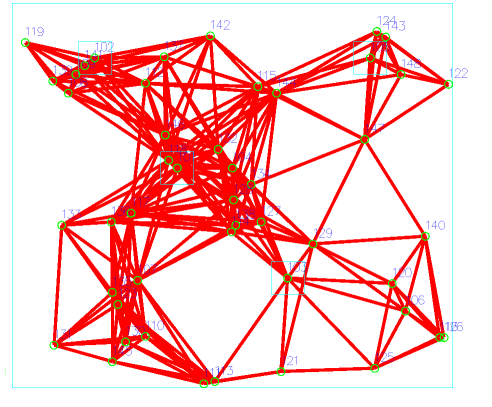
\includegraphics[width=0.5\textwidth]{oldWatcher.eps}
\caption{Watcher at start of project}
\end{figure}

\begin{figure}
\label{fig:legWatcherGUI}
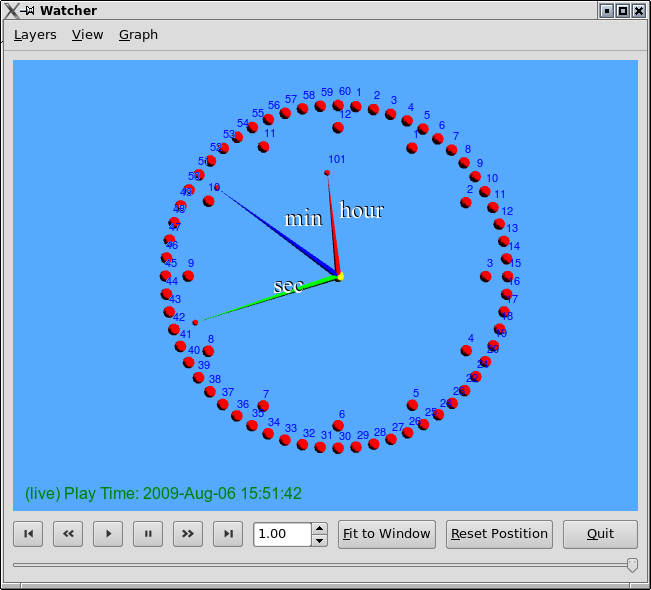
\includegraphics[width=0.8\textwidth]{legWatcherGUI.eps}
\caption{``Legacy Watcher'' at end of project. Note user interface widgets.}
\end{figure}

\begin{figure}
\label{fig:watcherWithBackground}
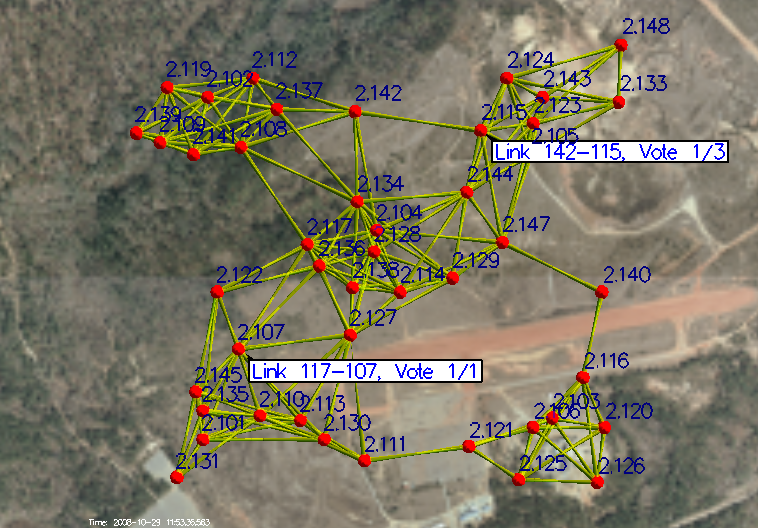
\includegraphics[width=0.8\textwidth]{watcherWithBackground.eps}
\caption{``Legacy Watcher'' showing background and 3D primitives}
\end{figure}

\begin{figure}
\label{fig:ogreWatcherGUI}
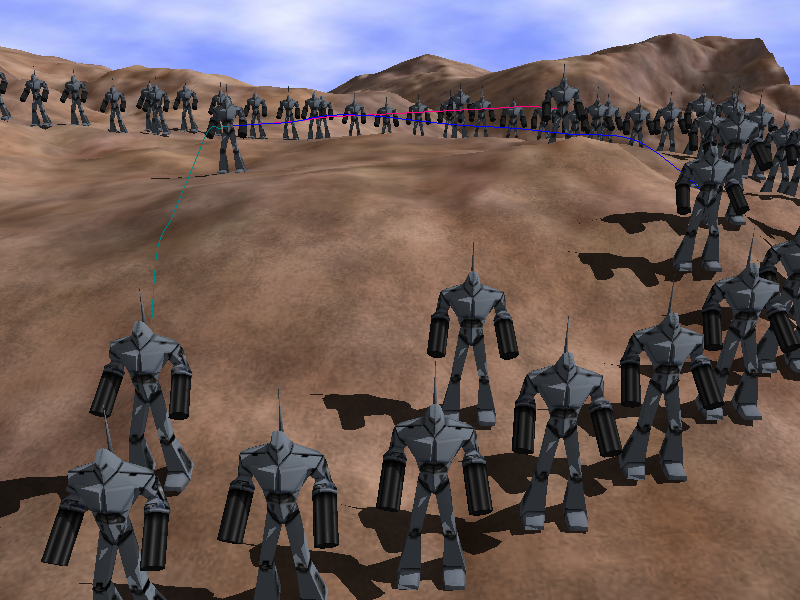
\includegraphics[width=0.8\textwidth]{ogreWatcherGUI.eps}
\caption{First cut at game engine-based watcher GUI. The watcher of the future?}
\end{figure}

\section{Lessons Learned}
We learned a lot of stuff, like totally.

\section{Recommendations for Future Work}
We should do some cool stuff in the future, like totally. 

\end{document}


